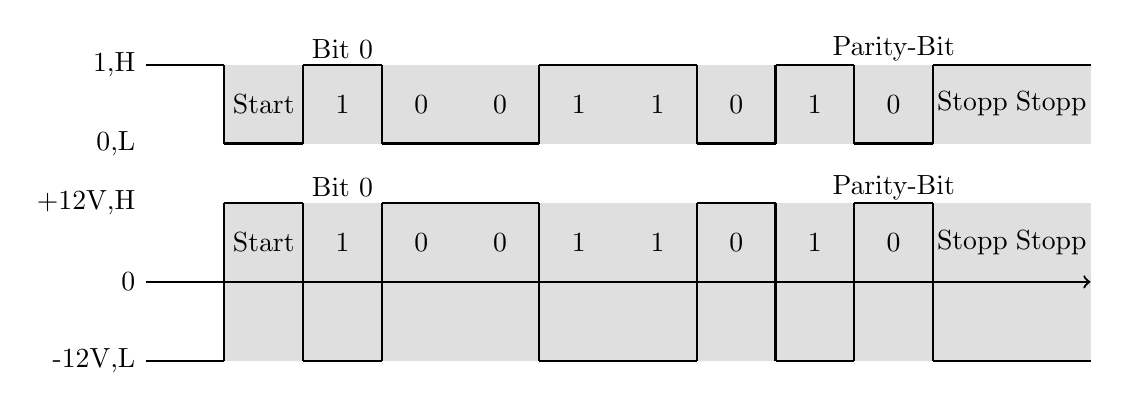
\begin{tikzpicture}[thick]
\fill [gray!25] (1,1) rectangle (12,0);
\foreach \x in {1,2,3,5,7,8,9,10}
	\draw (\x,0) -- (\x,1);
\foreach \x in {0,2,5,6,8,10,11}
	\draw (\x,1) -- ({\x+1},1);
\foreach \x in {1,3,4,7,9}
	\draw (\x,0) -- ({\x+1},0);
\foreach \x / \value in {2/1,3/0,4/0,5/1,6/1,7/0,8/1,9/0}
	\node at (\x+0.5,0.5) {$\value$};

\node at (0,1) [anchor=east] {1,H};
\node at (0,0) [anchor=east] {0,L};
\node at (1.5,0.5) {Start};
\node at (2.5,1.2) {Bit 0};
\node at (9.5,1.2) {Parity-Bit};
\node at (10.5,0.5) {Stopp};
\node at (11.5,0.5) {Stopp};

\begin{scope}[yshift=-50]
	\fill [gray!25] (1,1) rectangle (12,-1);
\foreach \x in {1,2,3,5,7,8,9,10}
	\draw (\x,-1) -- (\x,1);
\foreach \x in {0,2,5,6,8,10,11}
	\draw (\x,-1) -- ({\x+1},-1);
\foreach \x in {1,3,4,7,9}
	\draw (\x,1) -- ({\x+1},1);
\foreach \x in {2,5,6,8}
	\node at (\x+0.5,0.5) {$1$};
\foreach \x in {3,4,7,9}
	\node at (\x+0.5,0.5) {$0$};
\draw [->] (0,0) -- (12,0);

\node at (0,1) [anchor=east] {+12V,H};
\node at (0,0) [anchor=east] {0};
\node at (0,-1) [anchor=east] {-12V,L};
\node at (1.5,0.5) {Start};
\node at (2.5,1.2) {Bit 0};
\node at (9.5,1.2) {Parity-Bit};
\node at (10.5,0.5) {Stopp};
\node at (11.5,0.5) {Stopp};
\end{scope}
\end{tikzpicture}